%!TEX program = xelatex
\documentclass[UTF8]{ctexart}
\usepackage{ctex}

\usepackage{geometry}% 版面大小
\geometry{a4paper,scale=0.7}

\usepackage{graphicx}
\graphicspath{{assets/}}
\usepackage{caption2}
\usepackage{subfigure}
\usepackage{float}



\usepackage{listings}
\usepackage{xcolor}      %代码着色宏包
\usepackage{CJK}         %显示中文宏包

\usepackage[colorlinks,
            linkcolor=black,
            anchorcolor=blue,
            citecolor=green
            ]{hyperref}


\definecolor{mGreen}{rgb}{0,0.6,0}
\definecolor{mGray}{rgb}{0.5,0.5,0.5}
\definecolor{mPurple}{rgb}{0.58,0,0.82}
\definecolor{backgroundColour}{rgb}{0.95,0.95,0.92}

\lstdefinestyle{CStyle}{
    backgroundcolor=\color{backgroundColour},
    commentstyle=\color{mGreen},
    keywordstyle=\color{magenta},
    numberstyle=\tiny\color{mGray},
    stringstyle=\color{mPurple},
    basicstyle=\footnotesize,
    breakatwhitespace=false,
    breaklines=true,
    captionpos=b,
    keepspaces=true,
    numbers=left,
    numbersep=5pt,
    showspaces=false,
    showstringspaces=false,
    showtabs=false,
    tabsize=2,
    language=C
}

% \lstset{language=C}
% \begin{lstlisting}[style=CStyle]
% #include <stdio.h>
% int main(void)
% {
%    printf("Hello World!"); 
% }
% \end{lstlisting}

\title{\textbf{PA2-1 实验报告}}
\author{刘时宜 201180078}
\date{\today}

\begin{document}
\maketitle
\tableofcontents

\section{实现过程}
按照指令说的,不断重复跑测试样例、查看无效指令、对应查找反汇编结果确定指令类型、参考\verb|i386|手册实现函数、填入\verb|opcode.c|、跑测试样例的过程,直到完全跑完测试样例。

由于指令太多,具体实现过程就不在此报告中一一列举了。可以到以下两个连接中查看。

\href{https://andyliu92.notion.site/Instruction-Implementations-1-d3a43e548b98495998ed0eea963e749f}{Instruction-Implementations-1}

\href{https://andyliu92.notion.site/Instruction-Implementations-2-fe446e10733f47d08981711b9dc6f1a2}{Instruction-Implementations-2}

\section{对于一些指令实现讨论}

\subsection{LEA的实现}
这条指令的功能是将计算好的内存地址写到寄存器中。

这条指令在手册中被放在不能使用框架代码的指令列表中,但是若将源操作数作为一内存类型操作数,将目的操作数作为一寄存器类型操作数,在赋值是将源操作数的地址写入目的操作数的值,应当可以使用框架代码实现这个函数?

在实验中,按照上述思路实现代码,并未报错,代码如下:

\lstset{language=C}
\begin{lstlisting}[style=CStyle]
// @ pa_nju/nemu/src/cpu/instr/lea.c
#include "cpu/instr.h"
/*
Put the implementations of `lea' instructions here.
*/

static void instr_execute_2op()
{
    opr_dest.val = opr_src.addr;
    
    operand_write(&opr_dest);
}

make_instr_impl_2op(lea, rm, r, v)
\end{lstlisting}

\section{i386手册勘误}
\subsection{eip 在指令描述中的取值}
在指令的伪代码描述中(如下图),\verb|eip|的取值均为加上当前指令长度之后的取值,而非代码实现当中进入当前指令时的\verb|eip|的值。这点可能和芯片的电路实现有关,这样描述更加自然,但是在NEMU的代码中会造成一定困扰,或许可以在guide中做一点提醒?

\begin{figure}[H]
    \centering
    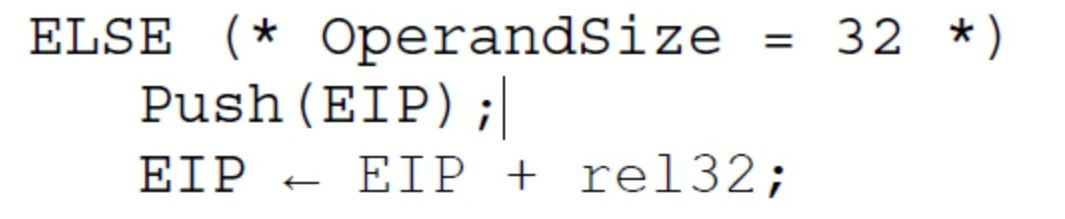
\includegraphics[width=0.4\textwidth]{1.jpg}
    \caption{call 指令中的伪代码}
\end{figure}


\subsection{Jcc 指令细节描述}
\verb|JNA|指令描述中,\verb|CF = 1|和\verb|ZF = 1|之间的逻辑关系(or)没有表达清楚,如下图:
\begin{figure}[H]
    \centering
    
\includegraphics[width=0.8\textwidth]{2.jpg}
    \caption{Jcc (JNA) 指令描述}
\end{figure}

正确表达式应当如\verb|JBE|指令的描述。
\begin{figure}[H]
    \centering
    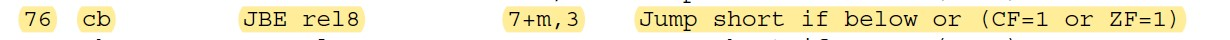
\includegraphics[width=0.8\textwidth]{3.jpg}
    \caption{Jcc (JBE) 指令描述}
\end{figure}

\subsection{MODr/m 位的解读}
\verb|MODr/m = 00 100|是手册上的描述里没有偏移量,如下图所示:
\begin{figure}[H]
    \centering
    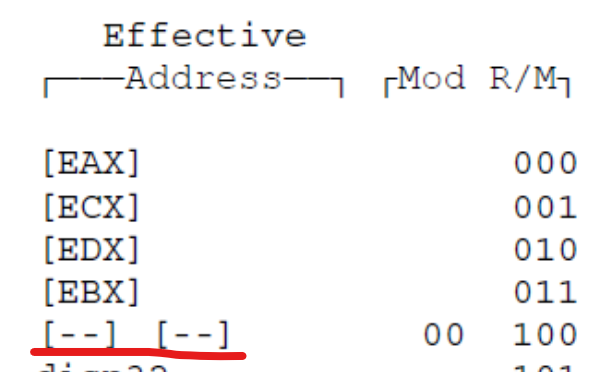
\includegraphics[width=0.5\textwidth]{4.png}
    \caption{MODr/m 描述}
\end{figure}

但是框架代码和反汇编结果均有32位偏移量:
\begin{figure}[H]
    \centering
    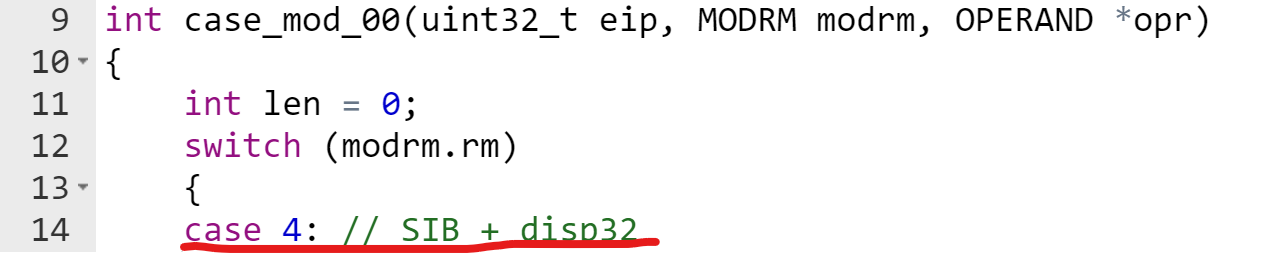
\includegraphics[width=0.5\textwidth]{5.png}
    \caption{框架代码实现}
\end{figure}

\section{思考题}
\begin{enumerate}
    \item 左侧为反汇编结果,右侧为\verb|.img|文件,对比可以看到,\verb|.img|文件的内容即为内存地址30000开始以后的内容。
    \begin{figure}[H]
        \centering
        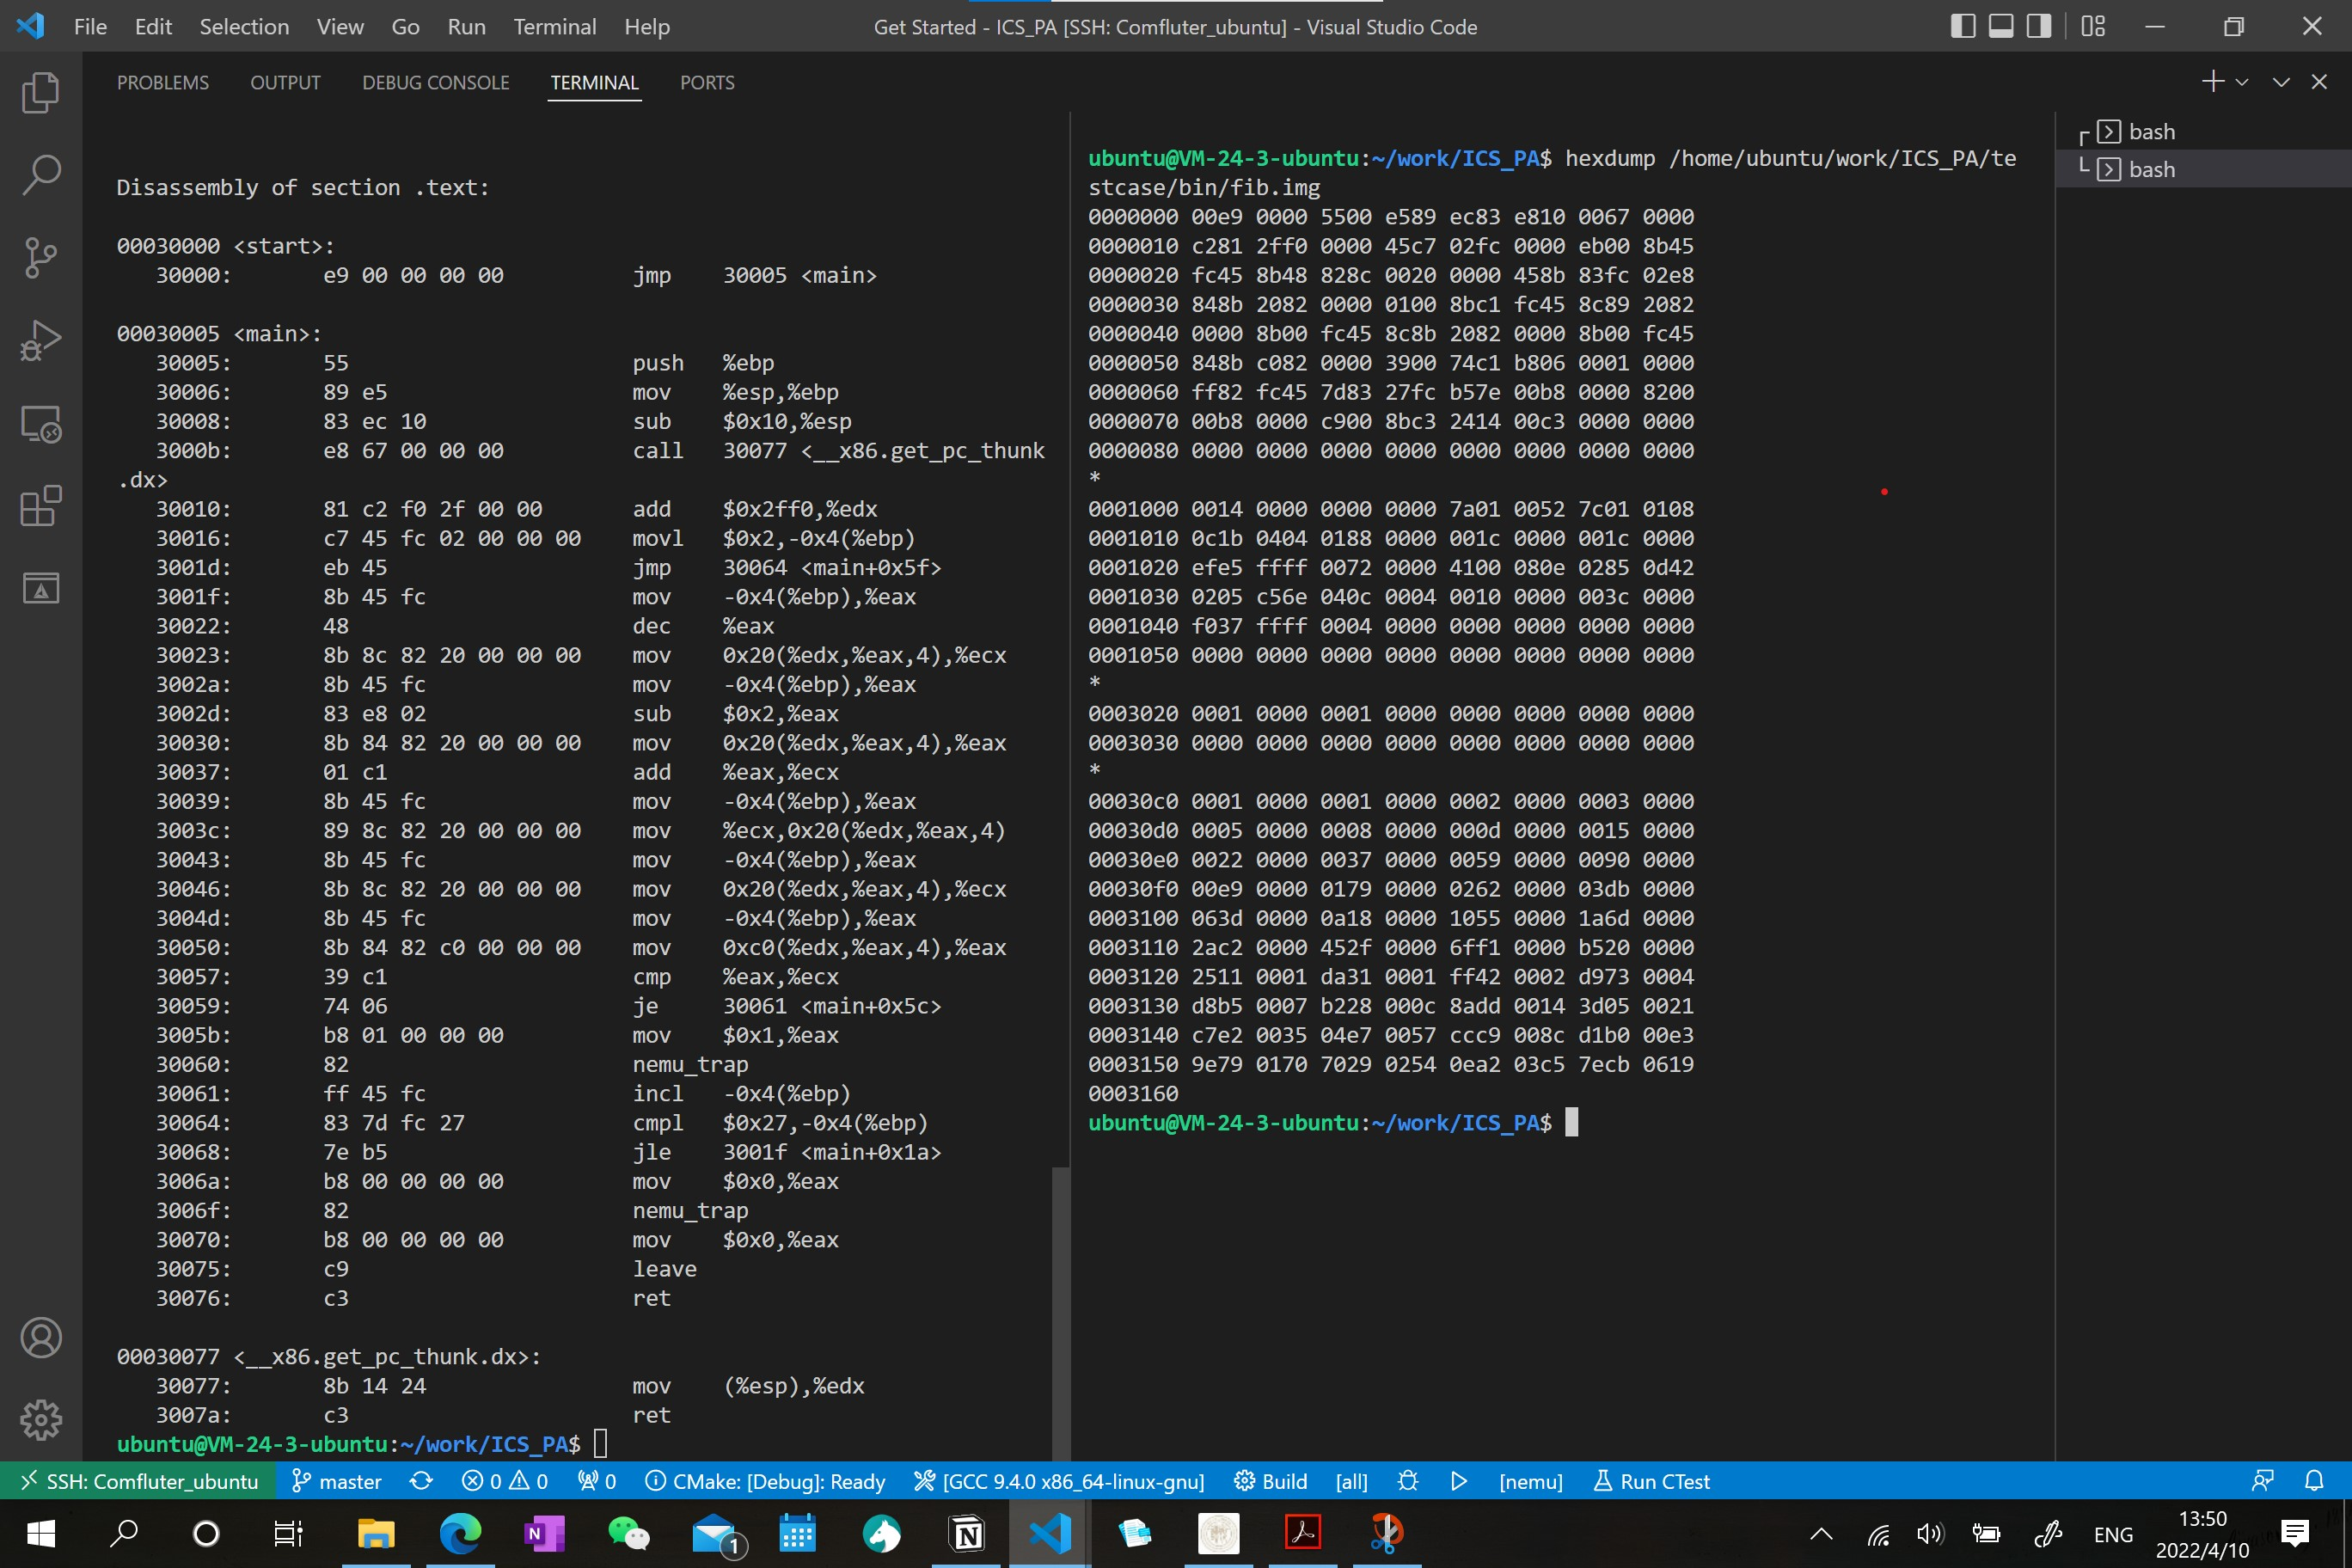
\includegraphics[width=0.8\textwidth]{6.jpg}
        \caption{框架代码实现}
    \end{figure}
    指令在机器中的表示为一串位串。
    \item 会使得\verb|instr_execute_2op()|函数全局可见,导致重名或者函数引用关系混乱。
    \item 由于这个测试样例中有大量浮点数运算,猜测为浮点数运算导致的精度损失造成的不能通过测试样例。
\end{enumerate}

\section{心得体会}
\begin{enumerate}
    \item PA教程设计得很好,让我对于解读机器码的过程以及指令的执行过程有了很切身的体会。
    \item 让我学习到构建大型应用程序的时候应当遵循模块化的代码架构设计,能够极大地减少混乱的可能性。
    \item 让我认识到代码可复用性的重要性。通过宏定义实现代码极大地减轻了工作量。
\end{enumerate}



\end{document}

% \begin{lstlisting}[style=CStyle]
% 
% \end{lstlisting}